\section{Análisis funcional de la interfaz del \glsentryshort{bofus}}
\label{sec:ana_bofuss}

En esta sección, exploraremos en detalle el análisis funcional de la interfaz del \gls{bofus}, centrándonos específicamente en los binarios que componen su arquitectura. Estos binarios, conocidos como \texttt{ofdatapath} y \texttt{ofprotocol}, desempeñan un papel fundamental en la operativa básica de este switch de espacio de usuario.\\
\\
El \texttt{ofdatapath}, como su nombre sugiere, es responsable de procesar el plano de datos en el \gls{bofus}. Este componente se encarga de recibir, analizar y tomar decisiones en función de los paquetes que atraviesan su pipeline de procesado de paquetes. A través del parser, tablas de flujo, y tablas de métricas, el ofdatapath garantiza una transferencia de datos fluida y eficiente en el entorno OpenFlow. Por otro lado, el \texttt{ofprotocol} se ocupa del agente de control en el \gls{bofus}. Su función principal consiste en establecer la comunicación entre el controlador y el switch. A través del \texttt{ofprotocol}, el controlador y \gls{bofus} pueden intercambiar información sobre el estado del switch, enviar nuevas reglas de procesado de paquetes, o recopilar estadísticas. Este binario es quien habilita al controlador llevar a cabo una gestión centralizada y dinámica de las políticas de red, facilitando la adaptación y optimización de la infraestructura según las necesidades del entorno.\\


\subsection{Binario \texttt{ofprotocol}}

El binario de ofprotocol establece un canal seguro de comunicación entre el \textit{datapath} OpenFlow y el controlador remoto. Este conecta con el plano de datos mediante Netlink o TCP, y con el controlador remoto mediante TCP o SSL, actuando de proxy entre los dos mundos. Se quiere señalar el hecho de que el binario pueda comunicarse con el \textit{datapath} mediante TCP, dado que según el creador de la herramienta indica que esos dos binarios pueden trabajar desacoplados en máquinas diferentes y comunicarse a través de la red. Sin embargo, esta configuración no es muy común, dado que la comunicación entre \textit{datapath} y agente de control es crítica, y no admiten ni delays, ni perdidas.\\


\begin{lstlisting}[language= bash, style=Consola, caption={Interfaz CLI del binario ofprotocol},label=code:binofproto]
    ofprotocol [options] datapath controller[,controller...]
\end{lstlisting}
\vspace{0.5cm}

Uno de los parámetros obligatorios a la hora de invocar al agente de control, es qué \textit{datapath} se va a gestionar. Este se puede indicar de las siguientes formas.

\begin{itemize}
    \item \texttt{unix:file}, se indica un descriptor de un socket UNIX, el cual deber ser el mismo que se indique a la hora que ejecute el ofdatapath. Mediante este socket unix se comunicarán \textit{datapath} y agente de control.

    \item \texttt{tcp:HOST[:PORT]}, en este caso, también se puede conectar en red mediante puerto y dirección IP. Este tipo de identificación se usa cuando se quiere tener separado en máquinas diferentes \textit{datapath} y agente de control. El puerto que se emplea por defecto es el 6653.
\end{itemize}

En cambio, el parámetro del controlador es opcional, y solo soporta conexiones TCP. Para la conexión con el controlador se contemplan dos paradigmas diferentes para la conexión del controlador.

\begin{itemize}
    \item \texttt{out-of-band}: con esta configuración el tráfico OpenFlow utiliza una red privada para comunicarse con el controlador.

    \item \texttt{in-band}: con esta configuración el tráfico OpenFlow viaja por la misma red que la red de datos. Esta opción es la opción por defecto.
\end{itemize}

Para llevar a cabo la configuración manual del control in-band, es necesario realizar algunos pasos clave con antelación. En primer lugar, se requiere especificar la ubicación precisa del controlador al llamar al binario de ofprotocol. Esto asegurará una conexión adecuada entre el controlador y el agente de control. Además, es crucial configurar la interfaz de red como el puerto local OpenFlow, el cual permite que ofprotocol establezca una conexión efectiva con el controlador. El puerto local OpenFlow es un puerto de red virtual que actúa como puente entre los puertos físicos del switch y el controlador. Para lograr esto, se puede especificar el nombre de la interfaz de red asignada al puerto local mediante la opción \texttt{--local-port} en la línea de comandos del binario ofdatapath. Generalmente, si no se indica ninguna interfaz, será el propio binario quien genere una interfaz de tipo TUN/TAP con el nombre \texttt{tap0/tun0}. Siguiendo estos pasos, se puede configurar adecuadamente el control in-band.


\subsection{Binario \texttt{ofdatapath}}


La herramienta de ofdatapath representa una valiosa implementación en el ámbito de las datapaths OpenFlow. Esta herramienta, diseñada para funcionar en el espacio de usuario, tiene la capacidad de supervisar y gestionar una o más interfaces de red de manera eficiente. Estas interfaces actúan como canales de comunicación fundamentales a través de los cuales los paquetes de datos son transmitidos y reenviados según las políticas y reglas establecidas en las tablas de flujos (Ir a sección \ref{subsec:BOFUSS}). Gracias a esta funcionalidad, ofdatapath permite un control efectivo y granular a nivel de flujo de datos en la red, asegurando un enrutamiento adecuado y optimizado de los paquetes. Su flexibilidad y adaptabilidad a diferentes escenarios hacen de esta herramienta una elección preferida en entornos OpenFlow a la hora de hacer pruebas de concepto, donde se busca una implementación amigable y funcional de un agente OpenFlow. A continuación en el bloque de código \ref{code:binofdata} se indica la interfaz de comandos de este bibario.\\

\begin{lstlisting}[language= bash, style=Consola, caption={Interfaz CLI del binario ofdatapath},label=code:binofdata]
    ofprotocol [options] datapath controller[,controller...]
\end{lstlisting}
\vspace{0.5cm}

La combinación del binario ofdatapath junto con el binario ofprotocol da lugar a lo que se conoce como \gls{bofus} (Basic OpenFlow Software Switch), una solución integral de software switch \gls{sdn} OpenFlow. Al utilizar \gls{bofus}, se obtiene un control y gestión a bajo nivel de las interfaces de red, lo que permite una administración eficiente de los flujos de datos que atraviesan la pipeline de procesamiento del switch. Es importante destacar que, para acceder a estas interfaces de red, el binario generalmente requiere ejecutarse con privilegios de super usuario. Además, es relevante considerar la forma en la que estos binarios se comunican entre sí. Por lo general, esta comunicación se establece a través de un socket UNIX, permitiendo una conexión directa y eficiente entre ambos componentes. Sin embargo, también es posible establecer una conexión pasiva mediante TCP, ofreciendo una alternativa para la comunicación entre los binarios. Esta flexibilidad en los mecanismos de comunicación brinda opciones adaptativas y versátiles, permitiendo que \gls{bofus} se adapte a diferentes entornos y necesidades. \\
\\
A continuación, se indican algunos de los parámetros más importantes de la interfaz CLI del binario ofdatapath. Empezando por el único de ellos obligatorio, que es, cómo indicamos el punto de comunicación del plano de datos hacia el exterior, véase un agente de control, como por ejemplo el binario ofprotocol.\\

\begin{itemize}
    \item \texttt{punix:file}, escucha por una conexión en el descriptor del socket UNIX indicado.

    \item \texttt{ptcp:[port]}, escucha por conexiones TCP en el puerto determinado. Según la wiki de la herramienta, indican que el puerto por defecto es el 975, lo que en la práctica no es verdad\footnote{Se tuvo que modificar la wiki de la herramienta \url{https://github.com/CPqD/ofsoftswitch13/wiki/Ofdatapath-Manual/_history}}, es el 6653.
\end{itemize}

El valor del puerto por defecto se puede comprobar fácilmente, a continuación en las figuras \ref{fig:ofdata_1} y \ref{fig:ofdata_2}. Como se puede ver se lanza el binario de forma \textit{standalone} sobre la interfaz de loopback del sistema, y si comprobamos con la herramienta \texttt{lsof} los puertos TCP en esto de escucha en la Network namespace por defecto, se puede ver como el binario está utilizando el puerto 6653. Pero se puede ir un paso más allá, podemos ir al propio código fuente de la herramienta, y ver en que macro definen el puerto por defecto, lo cual se puede comprobar \href{https://github.com/CPqD/ofsoftswitch13/blob/master/include/openflow/openflow.h#LL75C1-L75C27}{aquí}.

%fig 1
\begin{figure}[ht!]
    \centering
    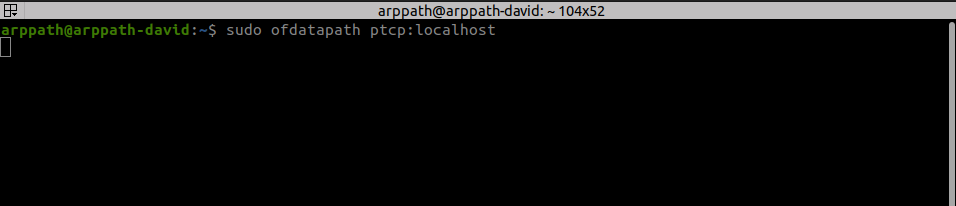
\includegraphics[width=\textwidth]{archivos/img/analisis/ofdata_1.png}
    \caption{Ejecución del binario \texttt{ofdatapath} en modo standalone}
    \label{fig:ofdata_1}
\end{figure}

%fig 2
\begin{figure}[ht!]
    \centering
    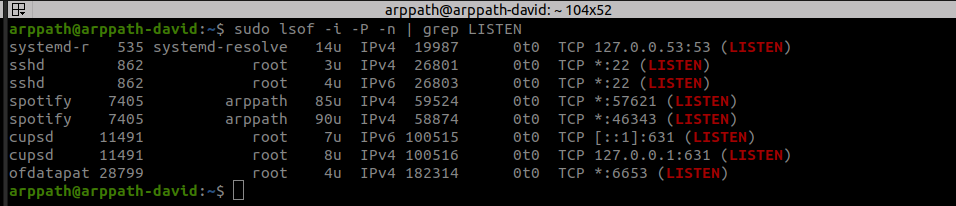
\includegraphics[width=\textwidth]{archivos/img/analisis/ofdata_2.png}
    \caption{Comprobación del puerto de  escucha del binario \texttt{ofdatapath}}
    \label{fig:ofdata_2}
\end{figure}


Sigamos con los parámetros de configuración del software switch. Uno de los más importantes, es indicar los puertos a gestionar el switch. Es decir, que interfaces va a manejar.

\begin{itemize}
    \item \texttt{-i, --interfaces=netdev[,netdev]}, Con este comando indicamos cada puerto que tendrá el switch. Cada interfaz se le asignará un número de puerto. Otro, detalle a tener en cuenta es que las interfaces no pueden tener IPs.

    \item \texttt{-L, --local-port=netdev}, Con este comando indicamos el puerto local que tendrá el switch el cual será la interfaz física o virtual, que se usará para el control in-band. Cuando está opción no está indicada, por defecto, se creará una interfaz de tipo tap, tap0 o algo así, la cual se utilizará para el control del software switch. Si no se quiere dejar como responsabilidad al Kernel la de asignar un nombre a la interfaz tap, se puede indicar como \texttt{--local-port=tap:name}. Se crea aquí. Para más información sobre las interfaces tun/tap, ver la sección \ref{linuxNetworking_tuntap}.

    \item \texttt{--no-local-port}, se le indica al software switch que no va a utilizar un puerto local, ergo, no podremos trabajar en modo in-band.

    \item \texttt{--no-slicing}, se utiliza para deshabilitar la configuración de las colas asociadas a los puertos. Por ello, contendrá un total de 0 colas. Esta opción se suele utilizar cuando algunas de las configuraciones de colas (tc y kernel) no se encuentran disponibles. (Mininet y Mininet-wifi corre el BOFUSS con esta opción por defecto).

    \item \texttt{-d, --datapath-id=dpid}, Especifica el Datapath ID Openflow, conocido como dpid. Es un identificador del datapath de 16 dígitos hexadecimales. Si no se especifica, el ofdatapath pilla uno aleatorio.
\end{itemize}